%!TEX root = ../../main.tex

\chapter{Fabrication of Nanodiamonds}	\label{ch::fabrication_nanodiamonds}
\chaptermark{Fabrication of Nanodiamonds}

"Diamond forms under high temperature and pressure conditions that exist only about 100 miles beneath the earth’s surface." (Homepage of the Gemological Institute of America Inc.)
	While this statement is true for natural gem diamonds, various methods exist to synthetically produce diamond for applications in industry and research. 
	In this chapter, different fabrication methods of \nds are explained.
	The first two procedures described are the \hpht method and the \cvd are described.
	These are the most commonly used fabrication methods for laboratory-produced diamonds. 
	The \hpht (\HPHT) process is similar to the natural growth process within earth and is widly used to synthetically produce diamonds for industry.
	Many measurements which are subject in this thesis are carried out on diamond produced with a \CVD process. 
	The third method mentioned is the wet-milling in a vibrational mill.
	The main focus of this thesis is on wet-milling \nds, which is a technique using \cvd or \HPHT diamond as starting material. 
	It has to be stressed, that in contrast to the other methods described in this chapter, the wet-milling process is not a process to produce diamond itself, rather it serves to crush a bigger diamond into pieces of  a desired size.
	For a more extensive list of diamond production processes refer for example to \cite{davis1993diamond}.
	Aside from the diamond production processes, the technical details of the \nds used for this thesis will be mentioned.
	% At the end, the methods of producing diamonds via detonation processes and sonicating graphite powders are briefly described.
	% As diamonds produced with this process is not scope of this thesis, they will only be shortly introduced to complete the list.

	

\section[HPHT]{High-Pressure High-Temperature Diamond}\label{sec::hpht}

	The \HPHT process was the first process with which diamond was successfully synthesized (in 1879).
	Depending on the exact process, temperatures and pressures are needed of a few thousand degrees Celsius and  \num{50000} to a few \num{100000}, respectively \cite{davis1993diamond}.
	Today, it is still widely used due to the relatively cheap production costs\cite{wikiSyntheticDiamond}.
	In this process, diamond is synthesized from graphite.
	For some forms of this method, a metallic solvent is added which lowers the needed pressures; the solvent causes the graphite to reach dissolve at lower pressures and temperatures, at the same time it causes the diamond to crystallize.
	The machine used for this kind of synthesis is a press.
	There exist several press designs, but they all provide a high temperature and a high pressure in their core.
	A disadvantage of the \HPHT process is that it the reachable size of the produced diamonds is limited.
	However, the advantage is, that \todo{HPHT advantage}
	\\
	In the scope of this thesis, \HPHT diamonds produced by Davydov et al. \cite{Davydov2014} were spectroscopically investigated.\todo{wie kommen da die SiVs rein?}


\section[CVD]{Chemical Vapor Deposition Diamond}\label{sec::cvd}

	\begin{figure}[tp]
		\begin{subfigure}[t]{ 0.49\linewidth}
			\caption{}\label{subfig::cvd_large}
			\centering
			\testbox{\includegraphics[trim = 0 0 0 0,  clip= true, height=5cm]{./pics/M05-13_191_131209_06.png}}
			% \caption{SEM picture of the milled nanodiamonds of a mean diameter of \SI{100}{\nano\meter}}
		\end{subfigure}
		\hfill
		\begin{subfigure}[t]{ 0.49\linewidth}
			\caption{}\label{subfig::cvd_detail}
			\centering
			\testbox{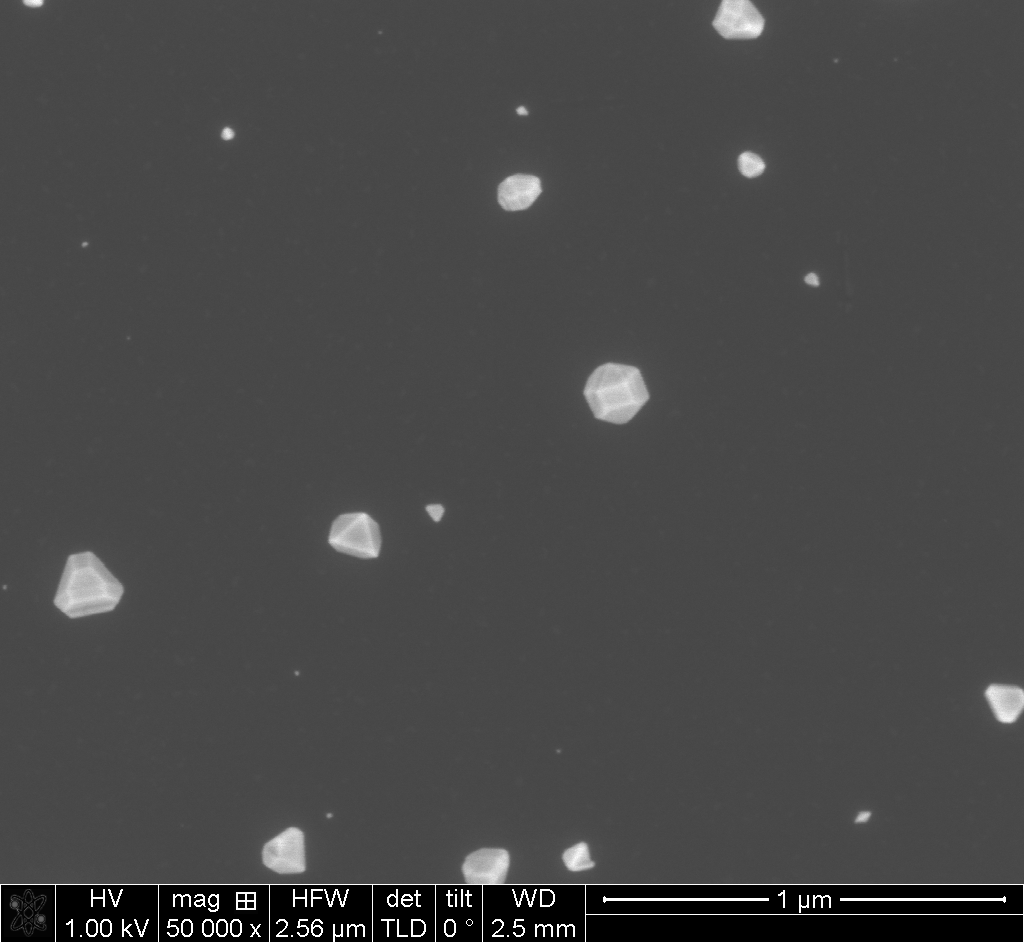
\includegraphics[trim = 0 0 0 0,  clip= true, height=5cm]{./pics/M05-13_191_131209_05.png}}
			% \caption{TEM picture of a \SI{100}{\nano\meter} diamond crystal.}
		\end{subfigure}
		\caption{}
		\label{fig::sem_cvd}
	\end{figure}

	\begin{figure}[tp]
		\centering
		\testbox{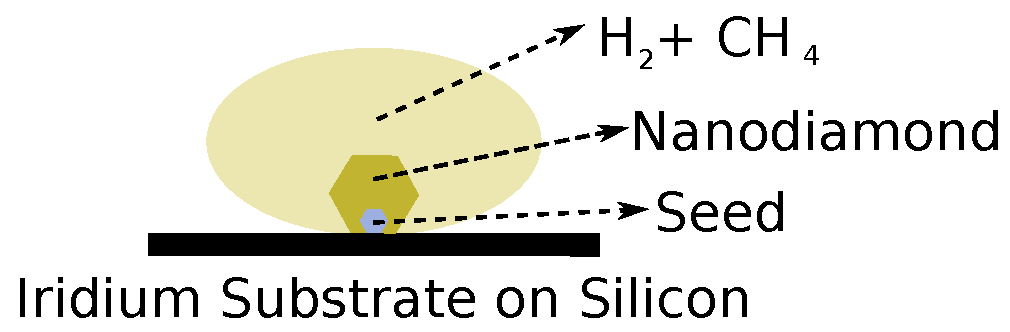
\includegraphics[trim = 0 0 0 0,  clip= true, width = 0.3\textwidth]{./pics/cvd_sketch.pdf}}
		\caption{Sketch showing the production of \CVD nanodiamonds in the growth chamber with a methane gas environment.}
		\label{fig::cvd_sketch}
	\end{figure}

	In contrast to the \HPHT process,  during the \cvd process, diamond is grown from a vapor phase.
	This process happens at moderate temperatures (\SIrange{700}{1300}{\celsius}) but very low pressures of less than \SI{1}{\bar} in a vacuum chamber \cite{}
	The diamond grows outside its stability zone and atomic hydrogen is necessary to suppress the simultaneous growth of graphite.
	The vapor phase within the growth chamber is a mixture of hydrogen and methane, the latter of which acts as a carbon source.
	Within the vacuum chamber, activation of the gas by an energy source (e.g. microwave plasma) breaks apart the gas molecules to release carbon atoms. 
	These atoms are drawn down toward the cooler substrate.
	On the substrate surface, various processes occur, such as adsorption, desorption and diffusion\todo{absatz zu ende bringen}.
	\\
	Growth on a substrate is easier, if the lattice constant of the substrate and the crystal to be grown are very similar.
	The lattice constant of \ir (\SI{0.384}{nm}\cite{Arblaster2010}) is very similar to the lattice constant of diamond (\SI{0.356}{nm}\cite{Davis1993}).
	Therefore, the diamonds were grown on a stratified substrate, consisting of \ir layers of \SIrange{60}{150}{nm} thickness grown onto an yttria-stabilized zirconia (YSZ) buffer layer, which in turn was grown on a silicon wafer \cite{Gsell2004a}.
	If the lattice constant of the substrate and the diamond are not matched, stress in the diamond lattice is induced.
	Therefore, the \ir substrate not only facilitates diamond growth, but also is a means to reduce unfavorable stress in the \nds (more on the effect of stress in \autoref{}).
	\\
	For crystals to form in a heteroepitactic growth (i.e. the substrate is another material than the grown crystal), a nucleation step is necessary \cite{Schreck2014a}.
	The easiest method to obtain nuclei on a substrate is to spin-coat the substrate with small diamond seed crystals of a size of a few nanometers. 
	This method is exploited for the production processes described in this section.
	Such small diamond crystals are commercially available, and are usually diamond particles produced by a detonation process.
	For the formation of these detonation diamond seeds, the high pressure produced by shockwaves of a detonation is used to create very small diamond particles of a size down to a few nanometers.
	During the \CVD growth process, carbon from the methane gas is adsorped\todo{is this correct?} to the seed crystals.
	To produce \nds of a desired size, the growth process is stopped when the diamond grown on the seed crystals reaches the desired size. 
	Otherwise, the individual crystals grow together to form diamond films, which is one possible of the starting material for the process descirbed in the next section (\autoref{sec::wet_milled_nds})
	\\

	% There are two major different ways to make a plasma from the gas in the chamber: microwaves or a hot filament.
	% While the hot filament is easy to be technically implemented, it has th{}e disadvantage that atoms which are etched from the filament during the growth process is likely to contaminate the diamond.
	% This circumstance can mess up a clean signal from \sivs.
	% Therefore, we preferred diamonds grown with in a microwave plasma.


	One of the advantages of the \CVD process is that \si can be incorporated \textit{in-situ}.
	This is achieved by the following process: \si from the substrate edges or sacrificial \si in the growth chamber is etched by the \verify{plasma} and \si atoms diffuse into the methane gas. 
	These atoms are then build into the diamond lattice while growth.
	After \nd growth, the \nds can be either investigated directly on the growth substrate or they can be shaken off in an ultrasonic bath to obtain a solution which can then be coated onto other substrates\todo{irgendwo einfuegen, was ich diesbezgl. gemacht hab}.
	\\
	In this thesis, two types of samples which were directly produced as nanodiamonds were investigated.
	The first batch (henceforth called \CVD samples) were grown on detonation diamond seeds (produced by the company Microdiamant, product Liquid Diamond monocrystalline, MSY {0-0.03} micron GAF) of a size smaller than \SI{3}{nm}.
	For the growth process, 1\% of methane was added to the hydrogen environment in the growth chamber.
	The growth process was performed with a pressure of \SI{30}{hPa} for \SIrange{30}{60}{min}, yielding \nds of a diameter of about \SIrange{100}{200}{nm}.
	\todo{put in figure}
	\\
	The other samples solely produced by a \CVD process are nanodiamonds grown onto molecular analogs of diamond crystals.
	A subgroup of these molecular diamonds are called diamondoids and are carbon crystals based on the carbon cage molecule adamantane \ch{C10H16}.
	The molecular diamonds used for this work are adamantane in cyclohexane, mercapto adamantane in cyclohexane, and cyclohexane.
	Each of these seed crystals was used in different growth processes.
	During the growth process, either 3\% or 1\% methane was added to the hydrogen plasma and either \si or \si dioxide was exploited to form \textit{in-situ} incorporated \sivs (see \autoref{tab::diamondiods}).


	\begin{table}[tp] 
		\centering 
		\caption{Summary of the samples grown on diamondoid seed crystals.} \label{tab::diamondiods} 
			\begin{tabular}{llll} 
			\toprule
			Sample name & Seed crystals & Methane conc. & \Si source \\ 
			\midrule
			160211\_E & Mercapto adamentane in cyclohexane & 1\% & \ch{SiO2} \\
			160211\_F & Cyclohexane                        & 1\% & \ch{SiO2} \\
			160212\_C & Cyclohexane                        & 3\% & \si         \\
			160212\_D & Adamentane in cyclohexane          & 3\% & \ch{SiO2} \\
			160212\_E & Mercapto adamentane in cyclohexane & 3\% & \ch{SiOs} \\
			160212\_F & Cyclohexane                        & 3\% & \ch{SiO2}\\
			\bottomrule
			\end{tabular} 
	\end{table}


\section[Wet-Milling]{Wet-Milled Nanodiamonds}\label{sec::wet_milled_nds}

	\begin{figure}[tp]
		\begin{subfigure}[t]{ 0.49\linewidth}
			\caption{}\label{subfig::sem_milled}
			\centering
			\testbox{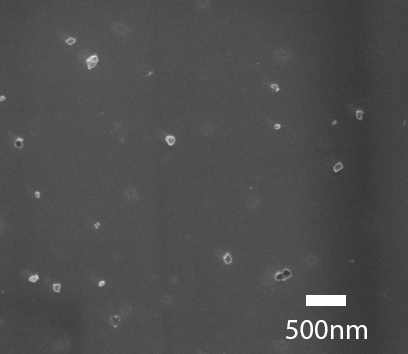
\includegraphics[trim = 0 0 0 0,  clip= true, height=5cm]{./pics/Ir27M_mitte_213_151111_22_crop.jpg}}
			% \caption{SEM picture of the milled nanodiamonds of a mean diameter of \SI{100}{\nano\meter}}
		\end{subfigure}
		\hfill
		\begin{subfigure}[t]{ 0.49\linewidth}
			\caption{}\label{subfig::tem_milled}
			\centering
			\testbox{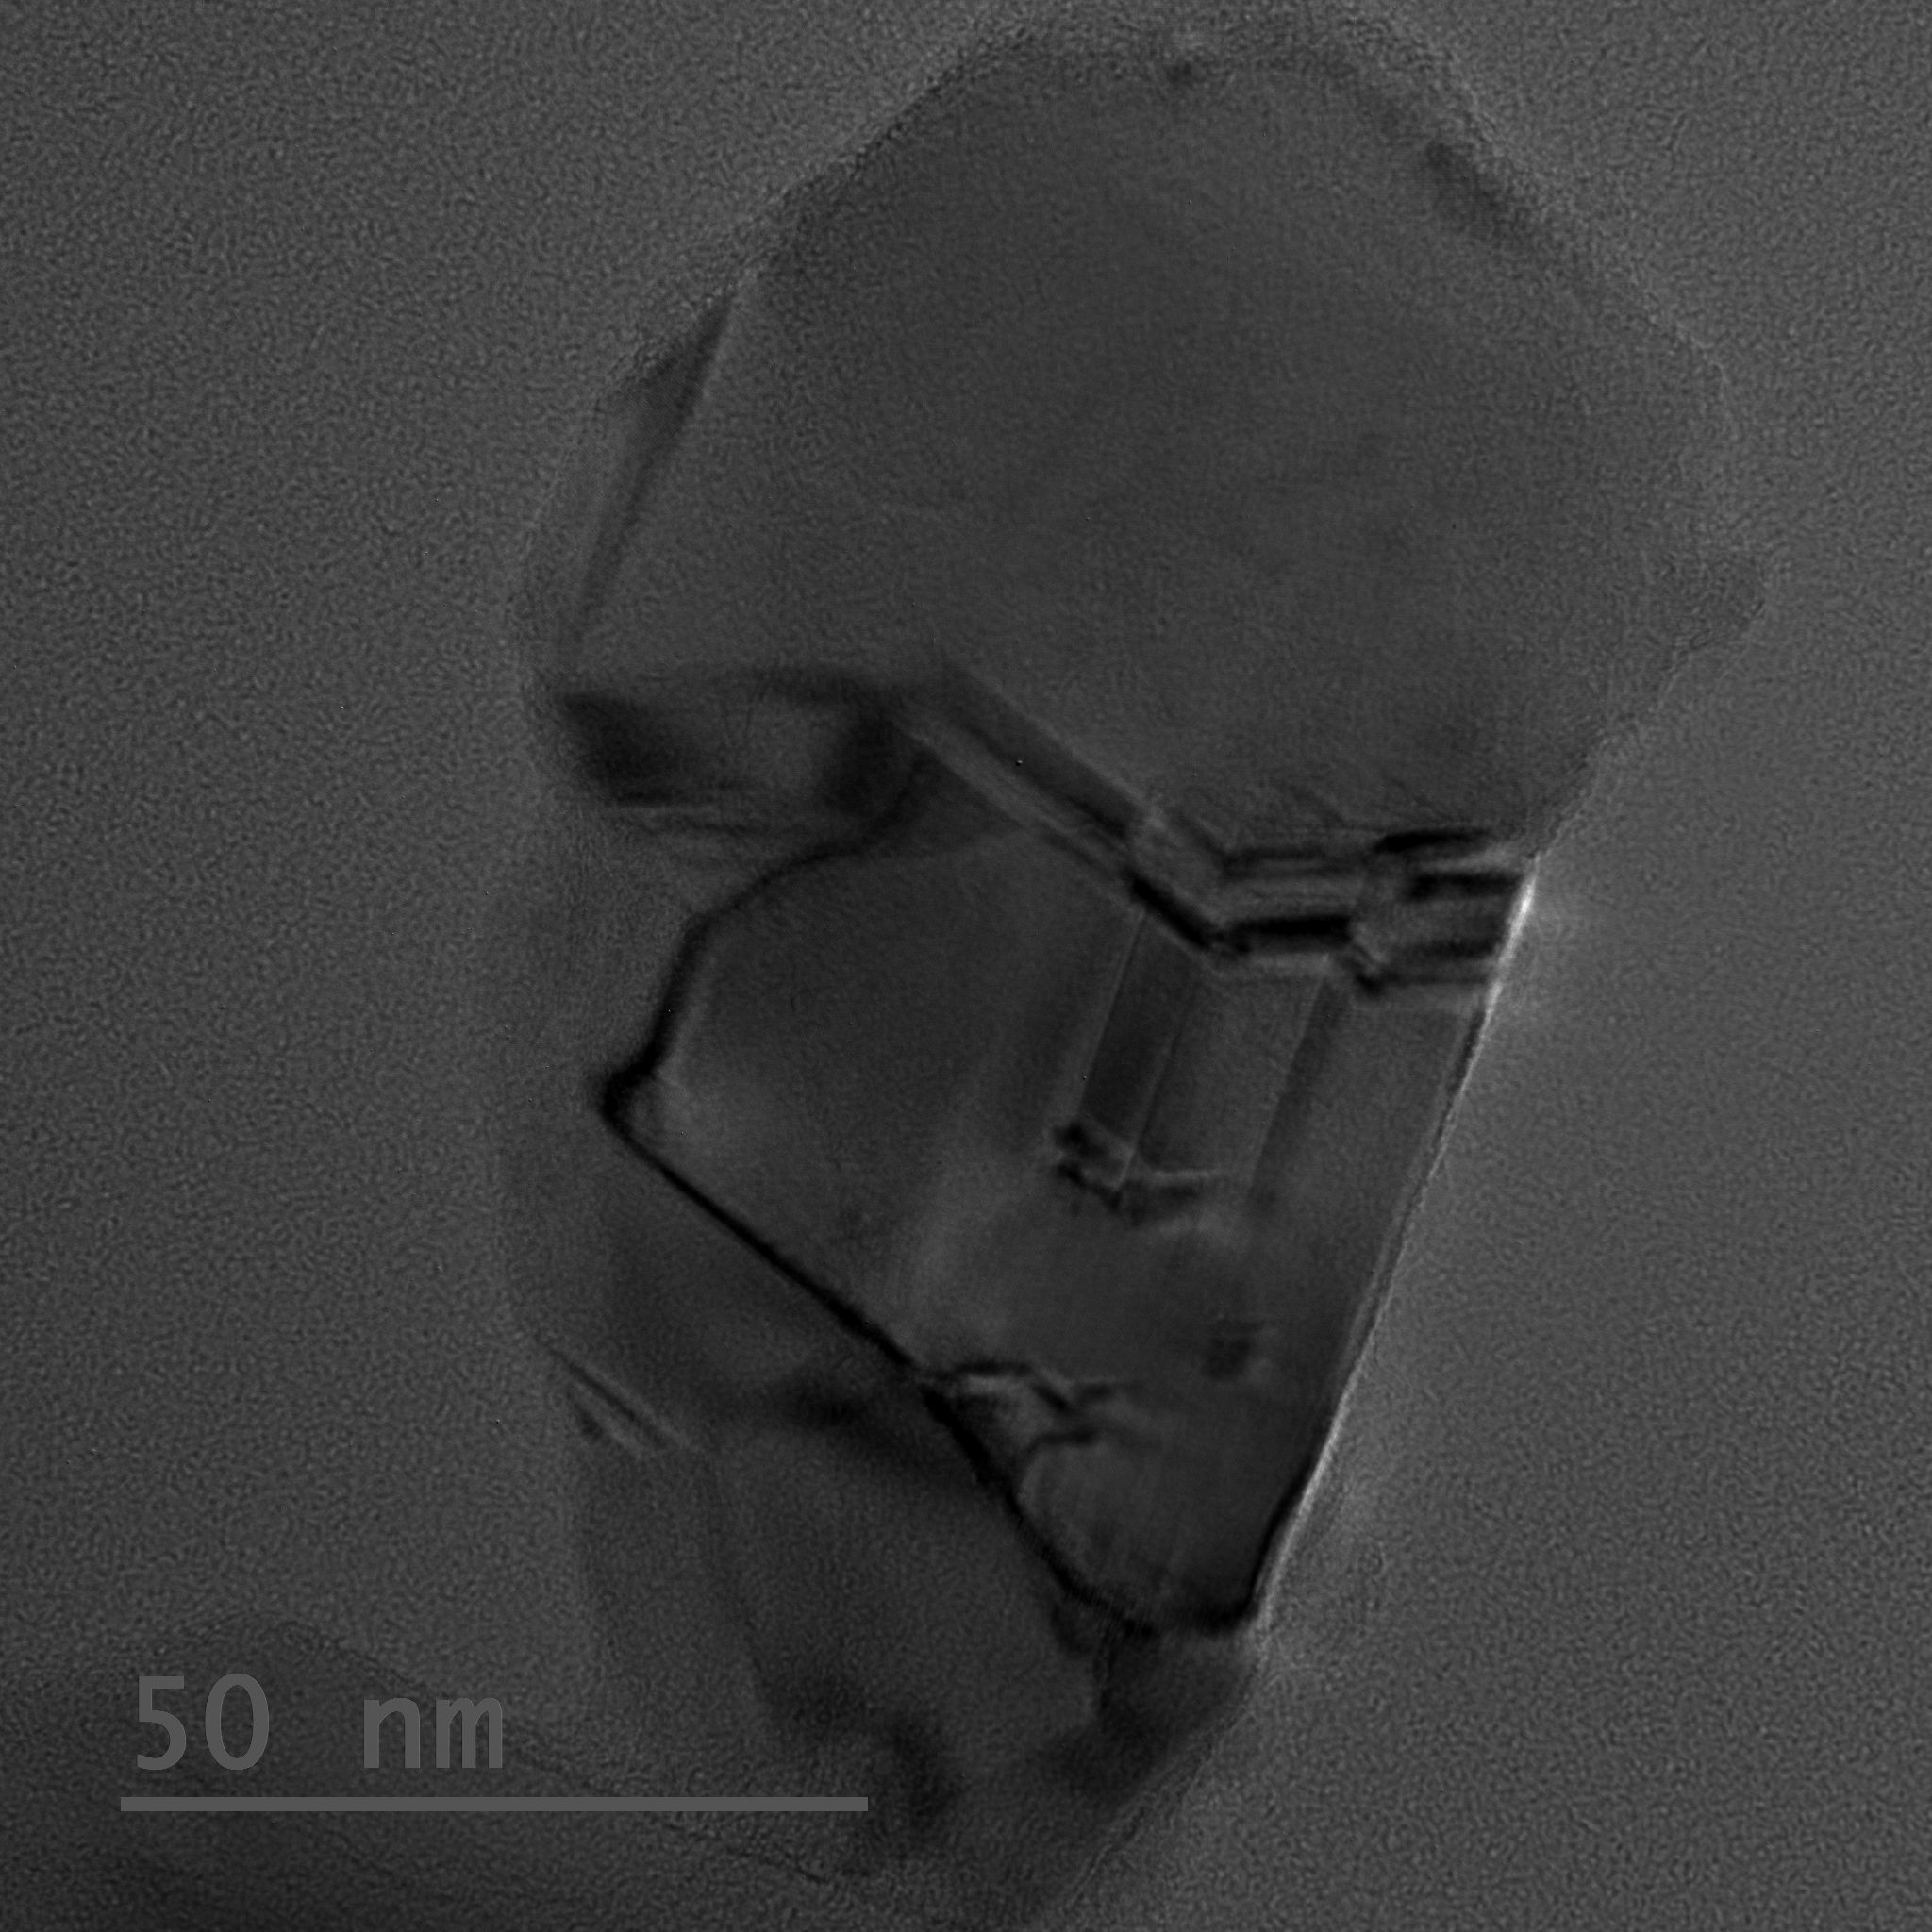
\includegraphics[trim = 0 0 0 0,  clip= true, height=5cm]{./pics/AM060-II-k4-2.png}}
			% \caption{TEM picture of a \SI{100}{\nano\meter} diamond crystal.}
		\end{subfigure}
		\caption{Pictures of the milled \nds (sample \insituH). (a) SEM picture showing the distribution of the \nd crystals on the \ir substrate. (b) TEM picture of a \nd particle.}
		\label{fig::semtem_millled}
	\end{figure}

	\begin{figure}[tp]
		\centering
		\testbox{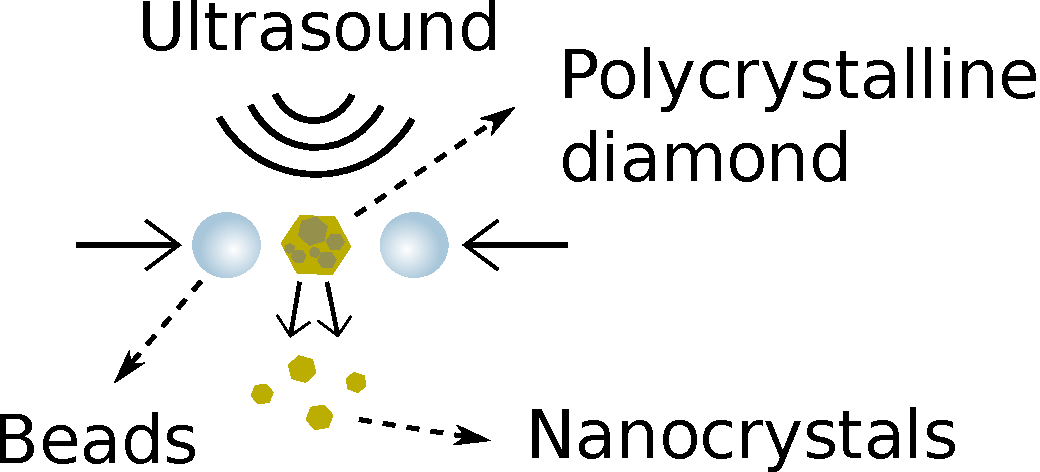
\includegraphics[trim = 0 0 0 0,  clip= true, width = 0.3\textwidth]{./pics/basd_sketch.pdf}}
		\caption{Sketch showing the \basd process. In a vibrational mill, vibrations from the mill drive the beads instead of the ultrasonic waves.}
		\label{fig::sketch_basd}
	\end{figure}

	Apart from growing \nds of a specific size directly via a \CVD process, macroscopic diamond starting material can be crushed to obtain small diamond particles.
	In contrast to \nds directly grown by a \CVD process, the process is divided into two sub-processes:

	\begin{enumerate}
		\item A macroscopic diamond has to be produced, for example by a \HPHT process or by \CVD growth.
		\item The macroscopic is milled to smaller diamond particles.
	\end{enumerate}

	To obtain the \nds investigated in this thesis, two different kinds of milling procedures were carried out: \basd (\BASD) and wet-milling in a vibrational mill.
	Both techniques use small beads to crush the diamond material. 
	The beads are either driven by ultrasonic waves (in the \BASD process) or by vibrations of the vibrational mill\todo{info about vibrational mill}.
	A sketch of the process is shown in \autoref{fig::sketch_basd}\todo{more info}.
	\\
	The big advantage of the milling process is that diamond nanoparticles can be produced in a very large quantity.
	When producing \nds directly via a \CVD process, the number of the produced \nds in one process scales with the surface of the substrate on which the \nds are grown.
	In contrast, the quantity of milled \nds scales with the volume of the starting material, therefore in one and the same process the limit for the obtainable amount of diamond nanoparticles is much higher.
	Another advantage of the milling process is that the \nds are in a aqueous solution after the milling process.
	Therefore, they can be used to spin-coat as-is onto any substrate suited for further experiments without further treatment.
	\\
	The disadvantage of the wet-milled \nds is that while as-grown \CVD \nds are technically single crystals, the milled \nds may contain grain boundaries \autoref{subfig::tem_milled}.
	While the polycristalline diamond film is more likely to break apart at grain boundaries, this fact is no guarantee that the resulting \nds do not contain grain boundaries, which is a reason for reduced crystal quality.
	\\
	\subsection{Wet-Milled \HPHT \Nds}\label{subsec::hpht_nds}
	In principle diamond produced by any production method can be used as starting material for the milling process.
	One way to distinguish the milled diamond samples is by classifying them according to the starting material.
	We investigated \nds, which were produced from a \HPHT starting material, milled by a wet-milling process and finally implanted with \ch{^{28}Si^1+} \todo{implantation parameters} from Dr. Detlef Rogalla at Ruhr-Universität Bochum (RUBION - Zentrale Einrichtung für Ionenstrahlen und Radionuklide).
	\\
	\subsection{\BASD \Nds}\label{subsec::basd_nds}
	For this thesis, two different batches of \nds produced by \basd were used.
	% - BASD SiV polykristalliner Diamant (Matthias Schreck) zermahlen von A. Krüger -> keine SiVs in NDs
	For one of the samples (\basds), a polycristalline diamond film was used as starting material.
	The diamond film was produced by the group of M. Schreck \cite{}.
	\Si was \textit{in-situ} incorporated during diamond growth, as described in \autoref{sec::cvd}.
	After milling, the \nds did not show any \pl from \sivs (see \autoref{}).
	We suspect that the reason for this is that \sivs are natural weak points of the diamond lattice which leads to a higher probablility for the diamond to break apart at areas where there are \sivs present.
	Hence a portion of the \sivs are destroyed by the milling process, especially if the target \nd size is of the same order as the individual crystals in the initial diamond film.
	\\
	%- BASD SiV: E6 die SiVs enthalten zermahlen (A. Krüger) -> keine SiVs in ND
	The other sample \todo{wirklich basd oder wet-milled?}(\basdes) was produced from a commercially available diamond film, produced by the company Element Six.
	This specific diamond film already contained \si impurities\todo{was wurde weiter damit gemacht?}.
	Similar to sample \basds, the sample did not exhibit \siv luminescence.
	\\
	\subsection{Wet-Milled \cvd \Nds}\label{subsec::milled_nds}
	% - milled CVD diamond film (in-situ SiV)
	In the following paragraphs, details of the production processes of the investigated samples produced by a wet-milling a \CVD diamond film in a vibrational mill are described. 
	For an overview of the samples refer to \autoref{tab::samplenames}.
	The starting material for the wet-milled \nds was a nanocristalline diamond film \cite{Williams2006a} directly grown on a silicon wafer by \CVD. 
	A microwave hydrogen plasma containing 1\% methane was used to grow on purified \SI{5}{\nano\meter} nanodiamond seeds (produced by PlasmaChem).
	To induce \textit{in-situ} \siv creation, sacrificial \Si pieces are situated in the growth chamber.
	During diamond growth the \Si pieces are etched by the plasma and individual atoms are incorporated into the diamond lattice.
	The diamond film is then milled by a wet-milling process in a vibrational mill with steel beads to crystals of average diameters of \SIlist{50; 70; 100}{\nano\meter} (\autoref{subfig::sem}).
	The particle size was determined with laser diffraction spectroscopy.
	Transmission Electron Microscopy (TEM) pictures of the diamond crystals show that the milled \nds are polycristalline, exhibiting a typical size of single crystals of a few tens of nanometers.
	In \autoref{subfig::tem} a TEM image of a typical \nd is shown.
	Crystal boundaries have effects on the formation of color centers:
	\sivs are more prone to form at crystal boundaries \cite{Zapol2001}.
	The high amount of steel containment due to the steel beads is removed by extensive acid treatment.
	We also investigated \nds milled with silicon nitride beads, and found that the choice of material of the beads did not cause any spectroscopic difference.
	The aqueous solution containing the \nds is drop cast onto an \ir film on a \Si substrate.
	The \ir film of a thickness of \SI{130}{nm} is grown onto a buffer layer of yttria-stabilized zirconia (YSZ) whith in turn is grown onto a \Si wafer.
	The \ir surface has the advantage that it acts as an antenna and therefore enhances the collection efficiency of fluorescence light \cite{Neu2012a}.
	Prior to drop casting, the substrate was cleaned in Piranha solution (50\% sulfuric acid H$_2$SO$_4$, 50\% hydrogen peroxide H$_2$O$_2$) to enhance the surface hydrophilicity and therefore obtain a homogeneous distribution of diamonds on the surface.
	Post-procession treatment comprises either both annealing in vacuum at \SI{900}{\degreeCelsius} and consecutive \ox in air at a temperature of \SI{450}{\degreeCelsius}, or only one of the two methods.
	The duration for either treatment method was 3-6 hours.
	\\
	\subsection{Twice Wet-Milled Implanted \Nds}\label{subsec::2_milled_nds}
	% - 2x vermahlene, implantierte NDs (E6->MDs->NDs)
	For comparative measurements, we also investigated \nds with \sivs implanted after diamond growth. 
	For those \nds starting material was a polycristalline Element Six diamond film (electronic grade).
	In bulk material, the implantation causes the \sivs to form in a specific depth dependent on the implantation energy, leaving most of the diamond vacant of \sivs.
	As a consequence, a big portion of  \nds milled from such a bulk material would not host any \sivs.
	To obtain diamond particles with a homogeneous distribution of \sivs, the implanted \nds are produced in several steps. 
	First, the diamond film was milled to diamond particles of sizes of a few micrometers.
	In the second step, these microdiamonds were then densely spin-coated onto \ir substrates and implanted with \ch{^{28}Si^1+}(implantation energy \SI{900}{keV}, fluence \SI{e11}{\per\centi\meter\squared}) by Jan Klug at rubitec - Gesellschaft für Innovation und Technologie der Ruhr-Universität Bochum mbH.
	To eliminate damage from the implantation process, the diamonds were annealed in vacuum at \SI{900}{\degreeCelsius} for 3 hours and subsequently oxidized in air at \SI{450}{\degreeCelsius} also for 3 hours.
	At last, the micrometer sized diamond particles were milled to a size of \SI{250}{\nano\meter}.



	\begin{table}[tp] 
		\centering 
		\caption{Summary of the \BASD samples. The first column indicates the names of the samples, the second the starting material from which the \nds were milled by \basd.} \label{tab::samplenames} 
			\begin{tabular}{llll} 
			\toprule
			Sample name & Starting material \\ 
			\midrule
			\basds & polycristalline diamond film (M. Schreck) \\ \hline 
			\basdes & polycristalline diamond film (Element Six) \\ 
			\bottomrule
			\end{tabular} 
	\end{table}



	\begin{table}[tp] 
		\centering 
		\caption{Summary of the wet-milled samples. The first column indicates the names of the samples, the second the mean diameter of the \nds, and the third describes how the \si was incorporated into the diamond.} \label{tab::samplenames} 
			\begin{tabular}{llll} 
			\toprule
			Sample name & Size & Si incorporation & Post-processing \\ 
			\midrule
			\insituF & \SI{50}{nm} & \textit{in-situ} & \begin{tabular}[c]{@{}l@{}}series of individual samples \\ with diverse post-processing steps\end{tabular}\\ \hline 
			\insituS & \SI{70}{nm} & \textit{in-situ} & \begin{tabular}[c]{@{}l@{}}series of individual samples \\ with diverse post-processing steps\end{tabular}\\ \hline 
			\insituSn & \SI{70}{nm} & \textit{in-situ} &  \begin{tabular}[c]{@{}l@{}}no post-processing \\ subset of \insituS \end{tabular}\\ \hline 
			\insituSo & \SI{70}{nm} & \textit{in-situ} & \begin{tabular}[c]{@{}l@{}}oxidized in air at 450\textdegree C \\ subset of \insituS \end{tabular}\\ \hline 
			\insituH & \SI{100}{nm} & \textit{in-situ} & \begin{tabular}[c]{@{}l@{}}series of individual samples \\ with diverse post-processing steps\end{tabular}\\ \hline 
			\insituHao & \SI{100}{nm} & \textit{in-situ} & \begin{tabular}[c]{@{}l@{}}annealed in vacuum at 900\textdegree C, \\ consecutively oxidized in air at 450\textdegree C \\ subset of \insituH \end{tabular}\\ \hline 
			\implantedTao & \SI{250}{nm} & implanted & \begin{tabular}[c]{@{}l@{}}annealed in vacuum at 900\textdegree C, \\ consecutively oxidized in air at 450\textdegree C\end{tabular}\\ 
			\bottomrule
			\end{tabular} 
	\end{table}





\section{\Ir Substrate}\label{sec::ir_substrate}


\begin{figure}[tp]
	\begin{subfigure}[t]{ 0.49\linewidth}
		\caption{}
		\centering
		\testbox{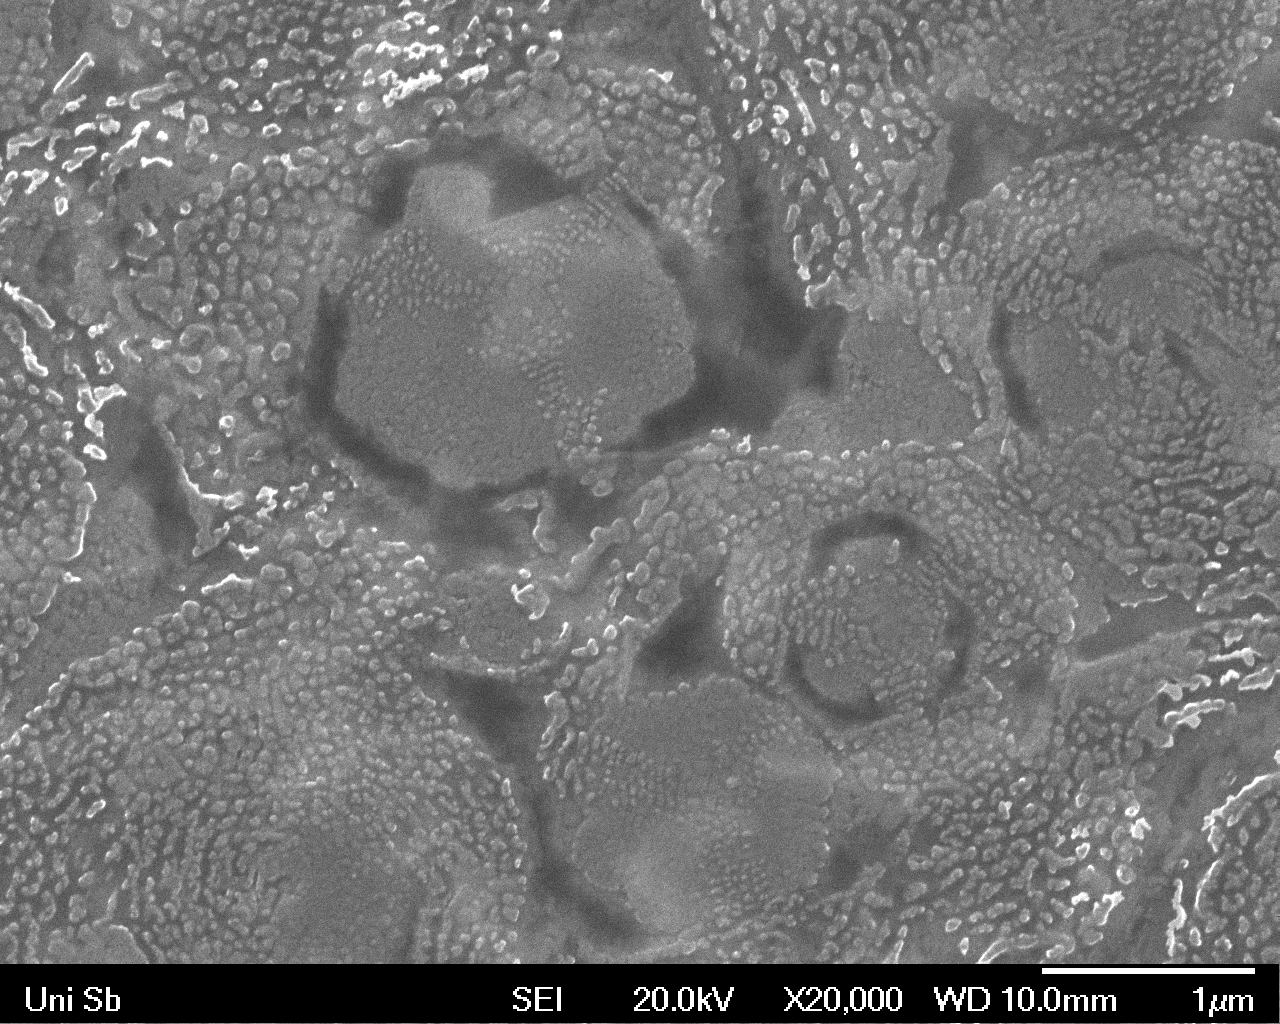
\includegraphics[trim = 0 0 0 0,  clip= true, width = \textwidth]{./pics/am21-sc-7-x20000-1.png}}
		\label{subfig::sunken_nd}
	\end{subfigure}
	\hfill
	\begin{subfigure}[t]{ 0.49\linewidth}
		\caption{}
		\centering
		\testbox{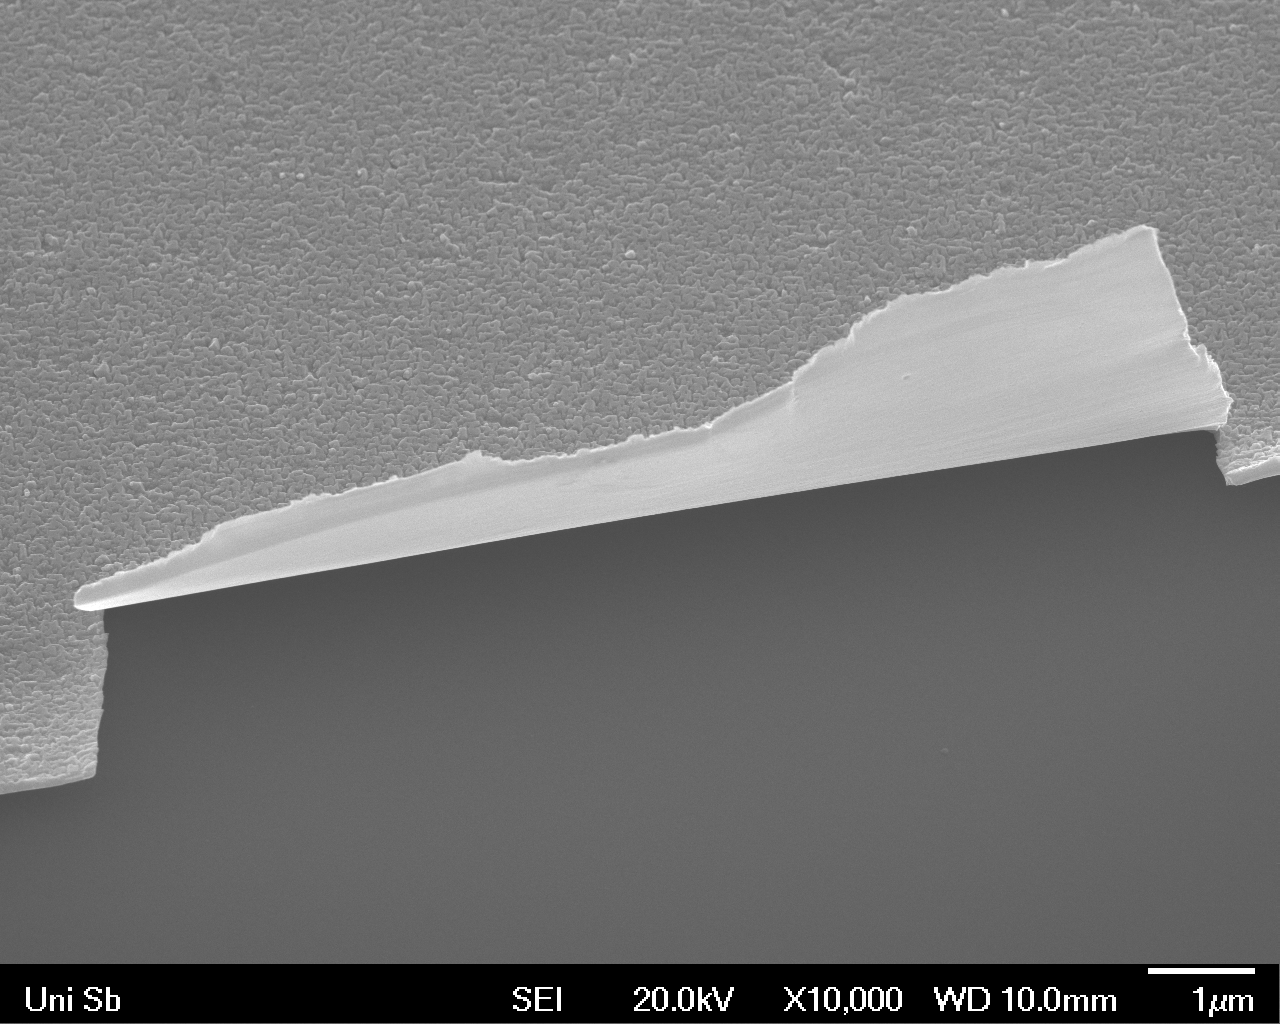
\includegraphics[trim = 0 0 0 0,  clip= true, width = \textwidth]{./pics/siq-basd-siv2-tilt45-x10000-1.png}}
		\label{subfig::peeled_ir}
	\end{subfigure}
	\caption{(a) SEM picture of \nds sunken into a \si substrate after annealing at \SI{900}{\celsius} for \SI{3}{h}. Magnification \num{20000} (b) SEM picture of an \SI{60}{nm} \ir layer that peeled off the substrate after an ultrasonic bath.}
	\label{fig::sem_substrates}
\end{figure}

	In \autoref{sec::cvd} it was already mentioned, that we used a \si substrate with an \ir layer on top in order to match the lattice constant of diamond.
	We also use the same substrates for the experiments with wet-milled diamonds, as the \ir has further advantages:
	\begin{itemize}
		\item The high hydrophility of \ir \todo{check numbers} enhances the homogenuity of the nanodiamonds on the substrate after spin-coating or drop-casting. 
		The hydrophility is further improved by treating the substrate in a Piranha etch (\todo{chem. Formel einfuegen}) by removing oxide layers on the surface. 
		The treatment with Piranha etch also has the advantage that all organic contamination is removed.
		Measurements after applying the Piranha cleaning yielded an estimation of the contact angle of slightly more than one degree.
		To find the contact angle, the volume of a water drop was compared to the surface it covered and an estimation of the contact angle deduced.
		\item During our post-processing steps, it is of major importance, that the substrate can withstand high temperatures.
		During one of our experiments with implanted nanodiamonds on a \si substrate, we encountered the problem that the \si sublimated and re-nucleated during annealing at \SI{1200}{\celsius}, causing the diamonds to sink into the \si surface \ref{fig::sunken_nd}.
		\Ir has a high melting point of \SI{2446}{\celsius}, compared to the melting point of \SI{1414}{\celsius}.
		Therefore, \ir is less prone to damage by high temperatures and withstands annealing procedures up to our standard annealing temperature of \SI{1200}{\celsius} without problems.
		\item Additionally to the mentioned technical advantages, the \ir surface has advantages for the following spectroscopic measurements: 
		It acts both as a mirror and as an antenna for the \fl light emitted by the \siv \cite{}.
		Therefore, the collection efficiency of the \fl light is enhanced.
	\end{itemize}
	These advantages of the \ir surface is only countered by one minor disadvantage:
	If the \ir layer is too thin, it tends to peel off the substrate \autoref{subfig::peeled_ir}.
	We encountered this problem during a cleaning procedure in the ultrasonic bath.
	However, this disadvantage is circumvented by using a thicker \ir layer.
	For our measurements, we used an \Ir layer of a thickness of \SI{120}{nm}, with which we did not encounter any mechanical problems.